% Basic setup
\documentclass[12pt,a4paper]{article} % Defines the document type as an article with 12pt font size on A4 paper.

% Importing packages
\usepackage[english]{babel} % Sets the document language to English, adjusting hyphenation and language-specific typographic rules.
\usepackage[lmargin=2.5cm,rmargin=2.5cm,tmargin=2.5cm,bmargin=2.5cm]{geometry} % Sets custom page margins: left/right 2.5cm, top 2.5cm, bottom 2.5cm.

% Loading packages
\usepackage{amsmath}
\usepackage{hyperref}    % Enables hyperlinks for references, URLs, and citations.
\usepackage{xcolor}      % Provides tools for defining and using colors.
\usepackage{graphicx}    % Allows inclusion of images and graphics.
\usepackage{caption}     % Customizes captions for figures and tables.
\usepackage{subcaption}  % Supports subfigures and subcaptions within figures.
\usepackage{minted}      % Enables syntax highlighting for code listings.
\usepackage[T1]{fontenc} % Ensures proper font encoding, important for correct character rendering. Don't touch this.
\usepackage{lmodern}     % Sets the font to something more modern and easy to read.
\usepackage{setspace}    % Provides control over line spacing.
\usepackage{csquotes}    % Improves handling of quotations.
\usepackage{setspace}    % Used to set line spacing
\usepackage{longtable,booktabs,array} % Packages for advanced table formatting.
\usepackage[
  backend=biber,
  style=apa,  
]{biblatex}  % Manages citations and bibliography with APA style.

\setstretch{1.5} % Sets line spacing

\definecolor{LightGray}{gray}{0.9}  % Defines a custom color 'LightGray' with 90% gray, used for the code block background.
\hypersetup{                        % Configures hyperlink colors and behavior.
  colorlinks=true,                  % Enable colored links instead of boxes.
  linkcolor={blue},                 % Sets link color to blue.
  filecolor={maroon},               % Sets file link color to maroon.
  citecolor={blue},                 % Sets citation link color to blue.
  urlcolor={blue}}                  % Sets URL link color to blue.

\addbibresource{assets/bib-template.bib} % Adds the bibliography file.

\title{Place Holder page titre}        % Sets the document title.
\makeatletter
\providecommand{\subtitle}[1]{%     % Custom command to add a subtitle.
  \apptocmd{\@title}{\par {\large #1 \par}}{}{}
}

\makeatother
\subtitle{Va être remplacée par celle sur Teams}  % Sets the document subtitle.
\author{Charles Bouthillier Paul Charvet William Hamilton Samuel Roy}% Sets the author's name.
\date{2025-12-12}                   % Sets the document date.

% \renewcommand{\familydefault}{\sfdefault} % Changes the default font to one without serifs

% From this point, the preamble ends and the actual content of the document starts.
\begin{document}
\pagenumbering{gobble} % Stops counting the pages from this point until changed again.
\maketitle
%\begin{abstract}
%This is the LaTeX template (\textbf{Version 1.1}) from the DH Lab of the University of Basel. It is suitable for Seminar Papers and Master's / PhD theses, but can be adapted to fit a variety of use cases. It was created by Stefan Freitag and is derived from the Quarto template, which is also available from the DH Lab.

%The abstract of your paper / thesis goes right here. It will appear on the cover sheet (very first page) of the PDF, together with the title, subtitle, author name and date.

%If you do not want your document to have an abstract, you can also simple delete the 'abstract' part (or comment it out) with all its content and the final document will be created without it.
%\end{abstract}
\begin{center}
    \vfill
    \begin{figure}[H] 
          \includegraphics[width=.8\linewidth]{./assets/Université_Laval_logo_et_texte.svg.png}
    \end{figure}
        \setcounter{figure}{0}
        
    Université Laval\\
    Facutlé de science génie\\
    Québec
\end{center}
\newpage
\renewcommand*\contentsname{Table des matières} % This controls the title of your table of contents.
{
\hypersetup{linkcolor=}
\setcounter{tocdepth}{5} % Sets the maximum sublevel to be displayed within the table of contents.

\tableofcontents
}
\newpage
\pagenumbering{arabic}\setstretch{1.5} % Overwrites the previous command, pages are counted as normal from this point.


\section{Vue CAD 3D explosée}
    \begin{figure}[H] 
	    \includegraphics[width=1.1\linewidth]{./assets/Explose.pdf}
    \end{figure}

\section{captures d'écran des enveloppes d'impression}

\subsection{Volumes Préférentiels X-Y}
    \subsubsection{Volume #1}    
    \begin{figure}[H] 
	    \includegraphics[width=1.1\linewidth]{./assets/XY_pref1.pdf}
    \end{figure}
    \subsubsection{Volume #2}
    \begin{figure}[H] 
	    \includegraphics[width=1.1\linewidth]{./assets/XY_pref2.pdf}
    \end{figure}

\subsection{Volumes Préférentiels Z}
    \subsubsection{Volume #3}    
    \begin{figure}[H] 
	    \includegraphics[width=1.1\linewidth]{./assets/Z_pref1.pdf}
    \end{figure}
    \subsubsection{Volume #4}
    \begin{figure}[H] 
	    \includegraphics[width=1.1\linewidth]{./assets/Z_pref2.pdf}
    \end{figure}

\section{Croquis à main levé}
    \subsection{Concept \#1: Samuel Roy}
    \begin{figure}[H] 
	    \includegraphics[width=1.1\linewidth]{./assets/Croquis_SR.pdf}
    \end{figure}
    \begin{par}
	    Explication du concept
    \end{par}
    \begin{figure}[H] 
	    \includegraphics[width=1.1\linewidth]{./assets/Signature_SR.jpg}
    \end{figure}

    \subsection{Concept \#2: William Hamilton}
    \begin{figure}[H] 
	    \includegraphics[width=1.1\linewidth]{./assets/Croquis_WH.pdf}
    \end{figure}
    \begin{par}
	    Explication du concept
    \end{par}
    \begin{figure}[H] 
	    \includegraphics[width=1.1\linewidth]{./assets/Signature_WH.jpg}
    \end{figure}

    \subsection{Concept \#3: Paul Charvet}
    \begin{figure}[H] 
	    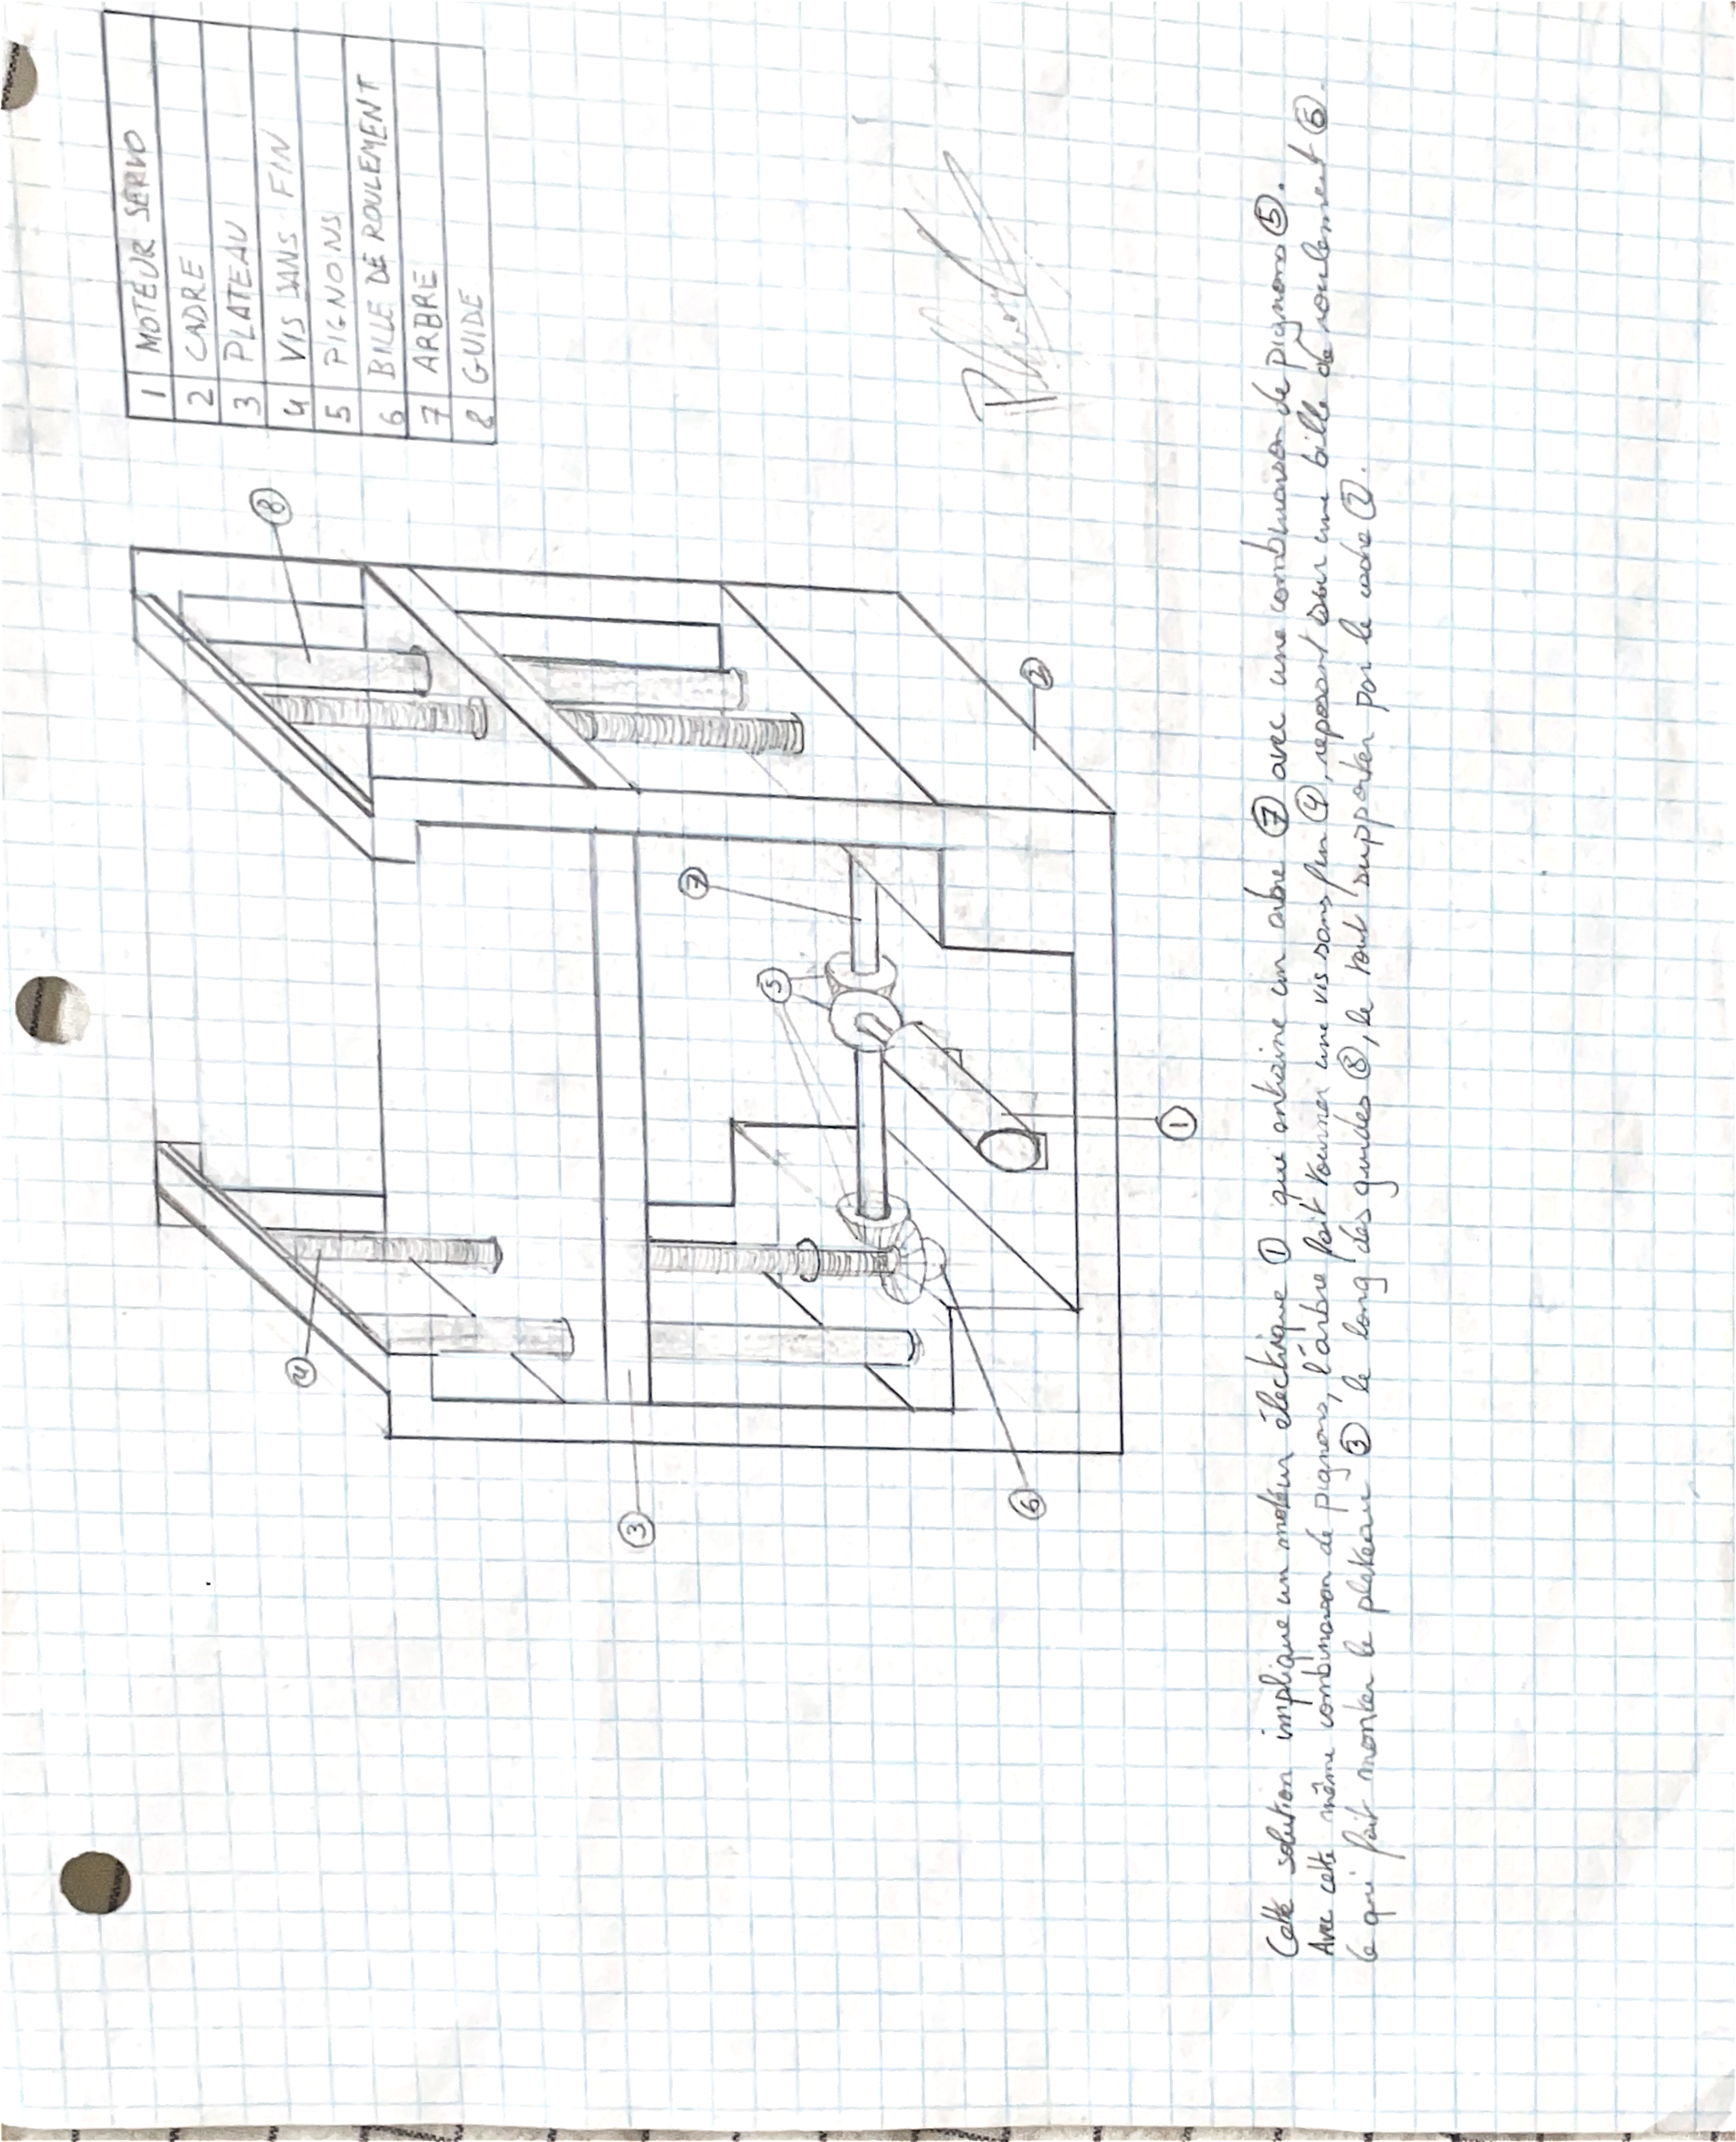
\includegraphics[width=1.1\linewidth]{./assets/Croquis_PC.pdf}
    \end{figure}
    \begin{par}
	    Explication du concept
    \end{par}
    \begin{figure}[H] 
	    \includegraphics[width=1.1\linewidth]{./assets/Signature_PC.jpg}
    \end{figure}

    \subsection{Concept \#4: Charles Bouthillier}
    \begin{figure}[H] 
	    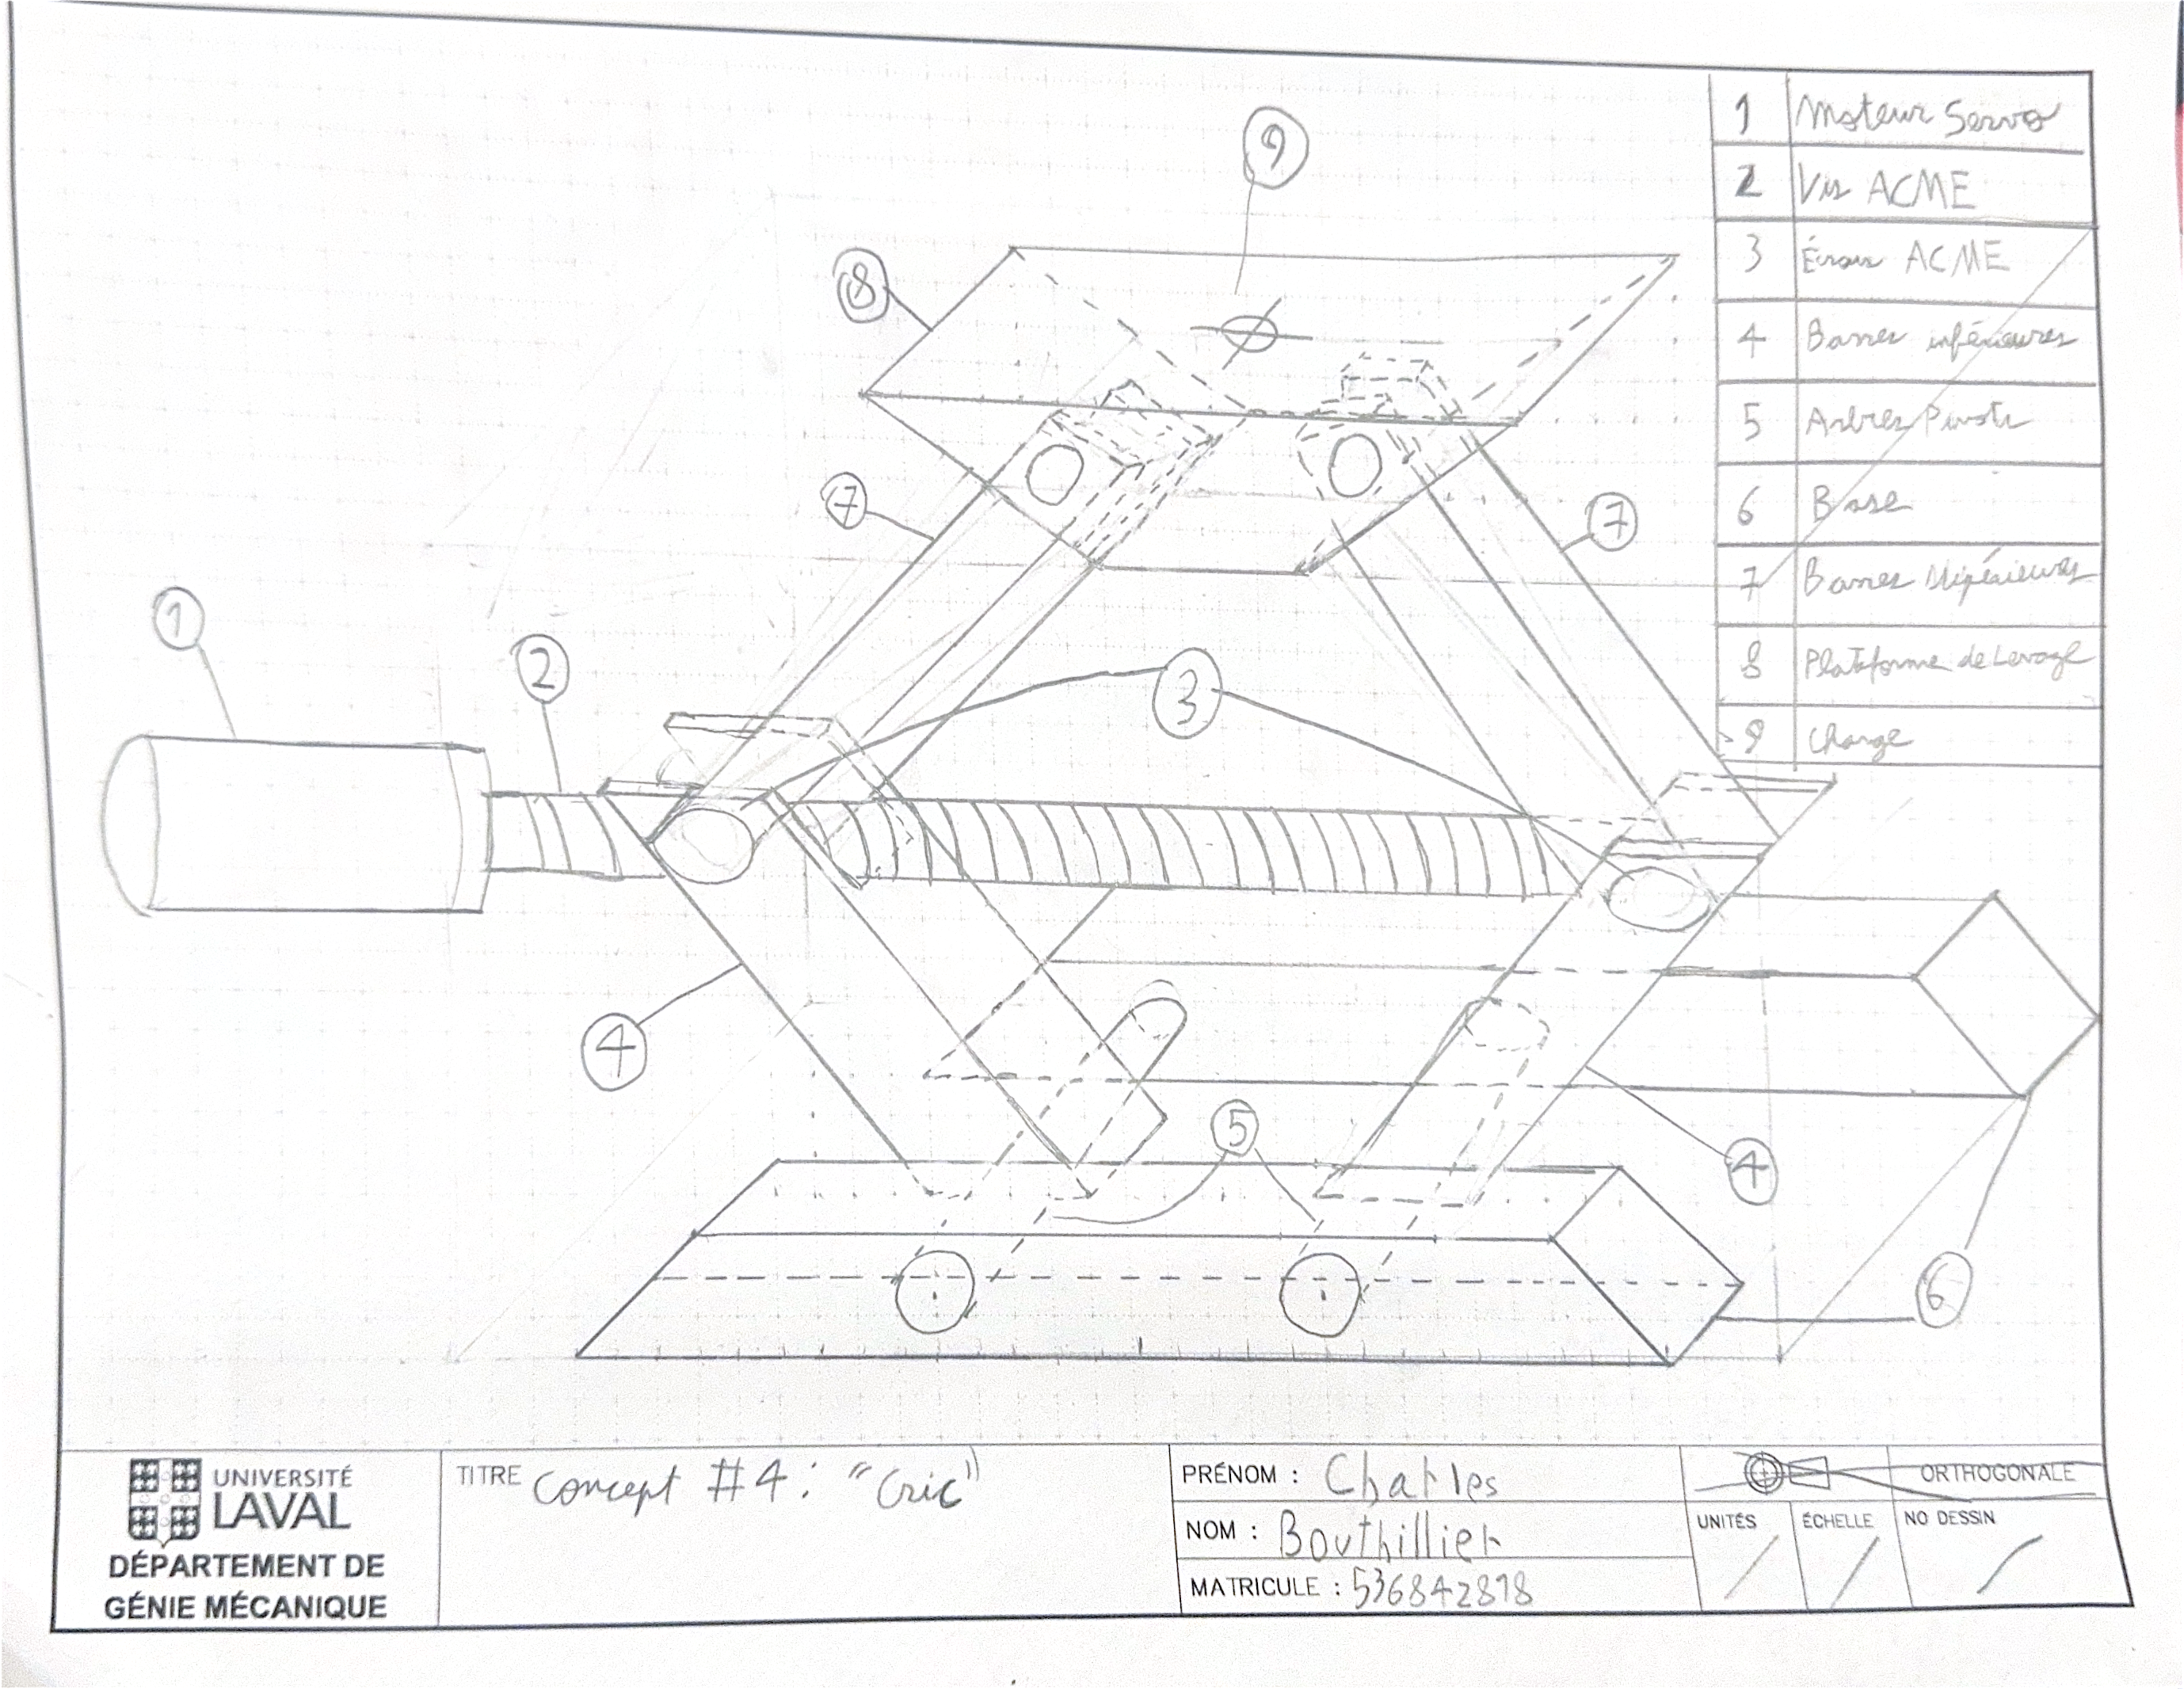
\includegraphics[width=1.1\linewidth]{./assets/Croquis_CB.pdf}
    \end{figure}
    \begin{par}
	    Explication du concept
    \end{par}
    \begin{figure}[H] 
	    \includegraphics[width=1.1\linewidth]{./assets/Signature_CB.jpg}
    \end{figure}
    
\section{Calculs}

\subsection{Calcul de faisabilité (\#1)}
\subsection{Calcul \#2}
\subsection{Calcul \#3}
\subsection{Calcul \#4}

\section{Conclusion}
    \subsection{Fiche de spécifications techniques}
    \begin{figure}[H] 
	    \includegraphics[width=1.1\linewidth]{./assets/Specs.pdf}
    \end{figure}
\newpage{}

\printbibliography[ % Prints the bibliography
heading=bibintoc,
title={References} % title of the 'references' section, change this if necessary
]

\end{document}
